% !TeX root = ../main.tex

\chapter{系统详细设计与实现}

在前两章中完成需求分析以及系统概要设计之后,本章将详细介绍各个功能
模块重难点的设计与实现。针对每一个功能模块,首先进行功能流程描述,然后对系
统实现类进行设计并阐述,通过类图介绍系统对象之间的交互顺序,最后进行系统实现的效果图展示。

\section{数据源管理}

数据源是入湖任务的前提要求,是Iceberg入湖任务的源头,注册相应数据源,创建入湖任务时即可根据创建的数据源选择对应的源表。
从数据源分类上来看,数据湖分析系统支持关系型数据库源(mysql)以及消息队列数据源(tube、kafka、pulsar),
该模块支持数据源创建、查看、编辑、删除功能。

在数据源管理中,用户首先需要登录系统。成功登录系统之后,进行数据源信息录入,基本信息包括
数据源名称和描述,不同的数据源所需要的详细信息也不一样,以关系型数据库MySQL为例,需
要配置mysql用户名、密码、库名、服务器地址和服务器端口。完成配置信息设置之后,会进行一个连接测试,测试是否能够连通,
接着会将数据源持久化保存在数据库中。活动图如图\ref{fig:创建数据源活动图}所示。

\begin{figure}[H]
  \centering
  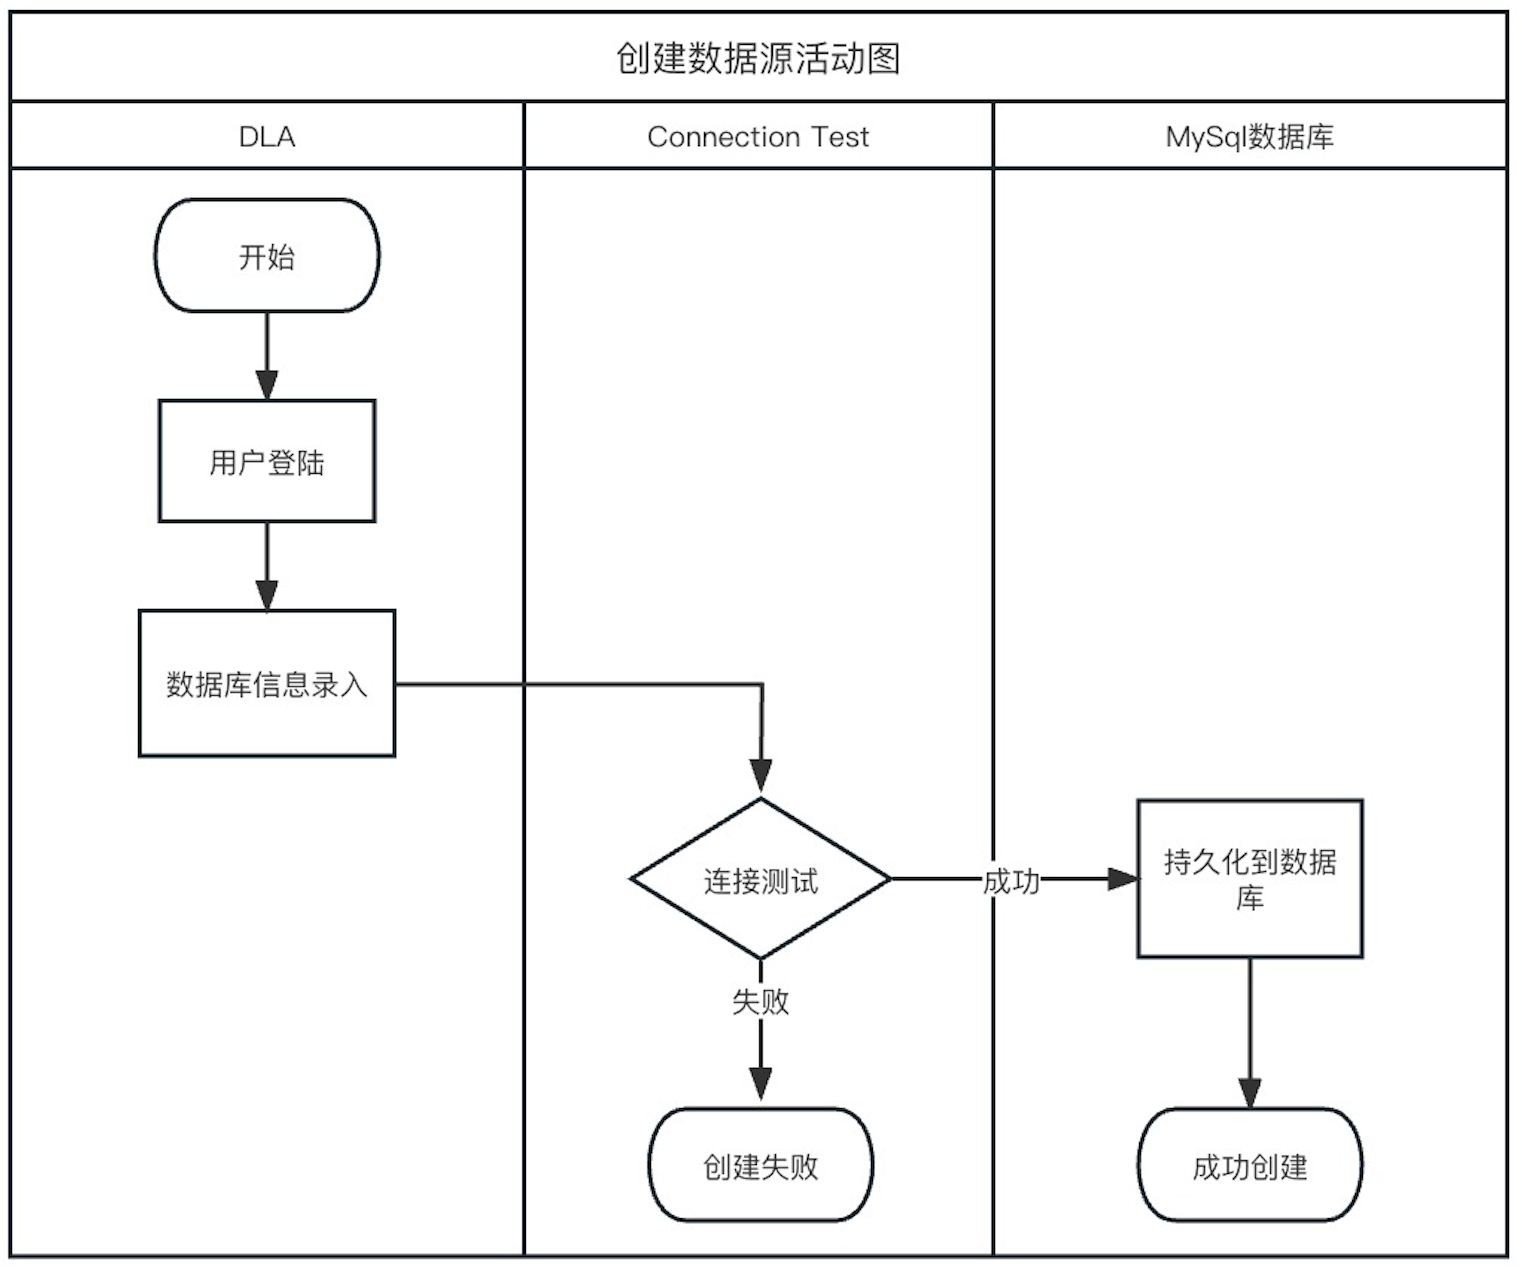
\includegraphics[width=0.85\textwidth]{创建数据源活动图.png}
  \caption{创建数据源活动图}
  \label{fig:创建数据源活动图}
\end{figure}

数据源管理是基于SpringBoot框架的Web应用,系统的主要类图如图\ref{fig:数据源类图}所示:

\begin{figure}[H]
  \centering
  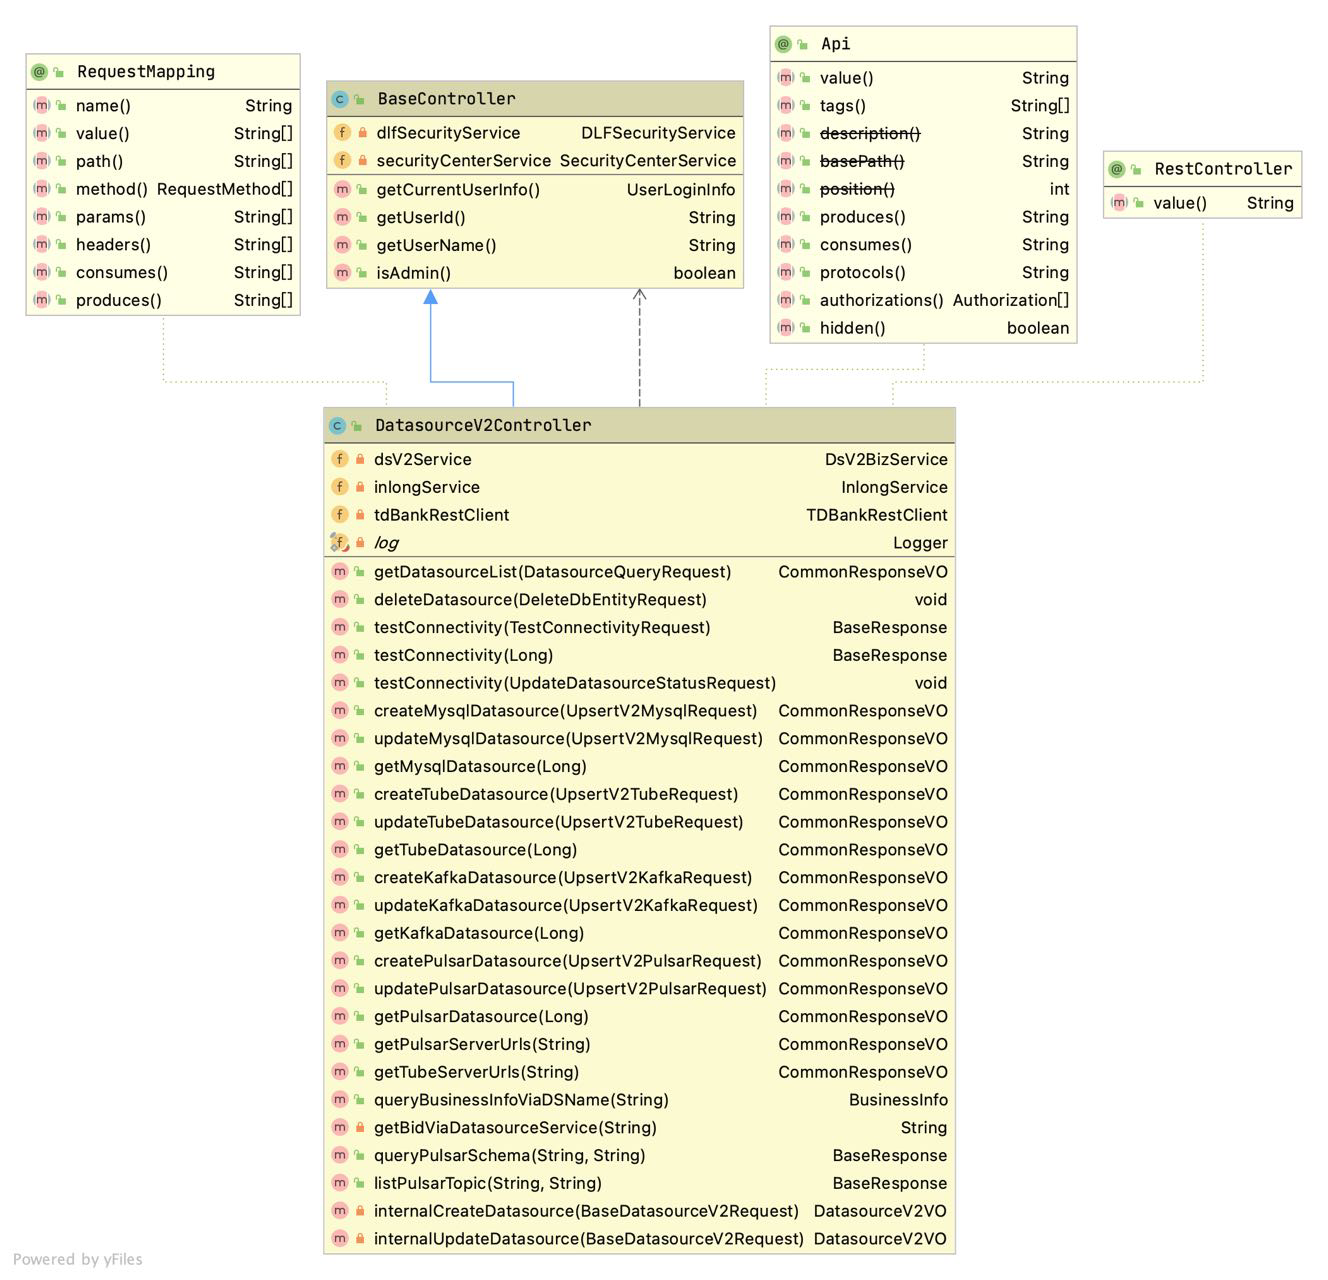
\includegraphics[width=1.0\textwidth]{数据源类图.png}
  \caption{数据源管理类图}
  \label{fig:数据源类图}
\end{figure}

其中,DatasourceV2Controller是数据源管理的核心类,是用户访问数据源管理的入口,
主要负责接受各种数据源的创建、查看、更新、删除以及连接测试的请求,对应的逻辑处理是在
成员变量DsV2BizService中实现的。

\section{元数据管理}

这里的元数据是描述Iceberg表的,Iceberg表即目标表,
是入湖任务的前提要求,可以创建新表或关联已有的表。元数据管理主要管理Iceberg元数据,
包括数据优化,表的创建、编辑、查看、删除,关联已创建的表,库的注册和查看。其中数据优化功能将单独介绍。表的创建可在数据湖分析
系统上创建新的Iceberg表,也可以关联在其他平台上已创建的Iceberg表。表的编辑支持对已创建的表进行
修改和编辑,包括增加和删除字段操作。

在元数据管理中,用户在对元数据进行操作前,都必须通过安全中心认证服务,
因为Iceberg元数据是存储在hive metastore中的,而对hive metastore中的元数据修改在企业内
是比较敏感的,所以必须添加身份认证以及权限认证来确保安全问题。
以Iceberg表的创建和修改来说,表的创建需要和hive metastore、mysql进行交互,填写好基本信息并点击创建后,除了会判断
metastore中是否已存在表,若metastore中不存在,则会在metastore中创建实际的Iceberg表元数据,
还会判断MySQL中是否存在对应的DB和table,这里MySQL中的DB和
table实质上是一个映射,是用来方便在数据湖分析系统中展示表元数据的,若MySQL中不存在,则创建对应的DB和table;
表的修改如果涉及到字段的增加及删除操作,则会更新hive metastore中对应的表元数据,
这其中涉及到的对metastore进行操作前都会进行安全中心的身份认证和权限认证。创建Iceberg表活动图如图\ref{fig:表元数据创建活动图}所示。

\begin{figure}[H]
  \centering
  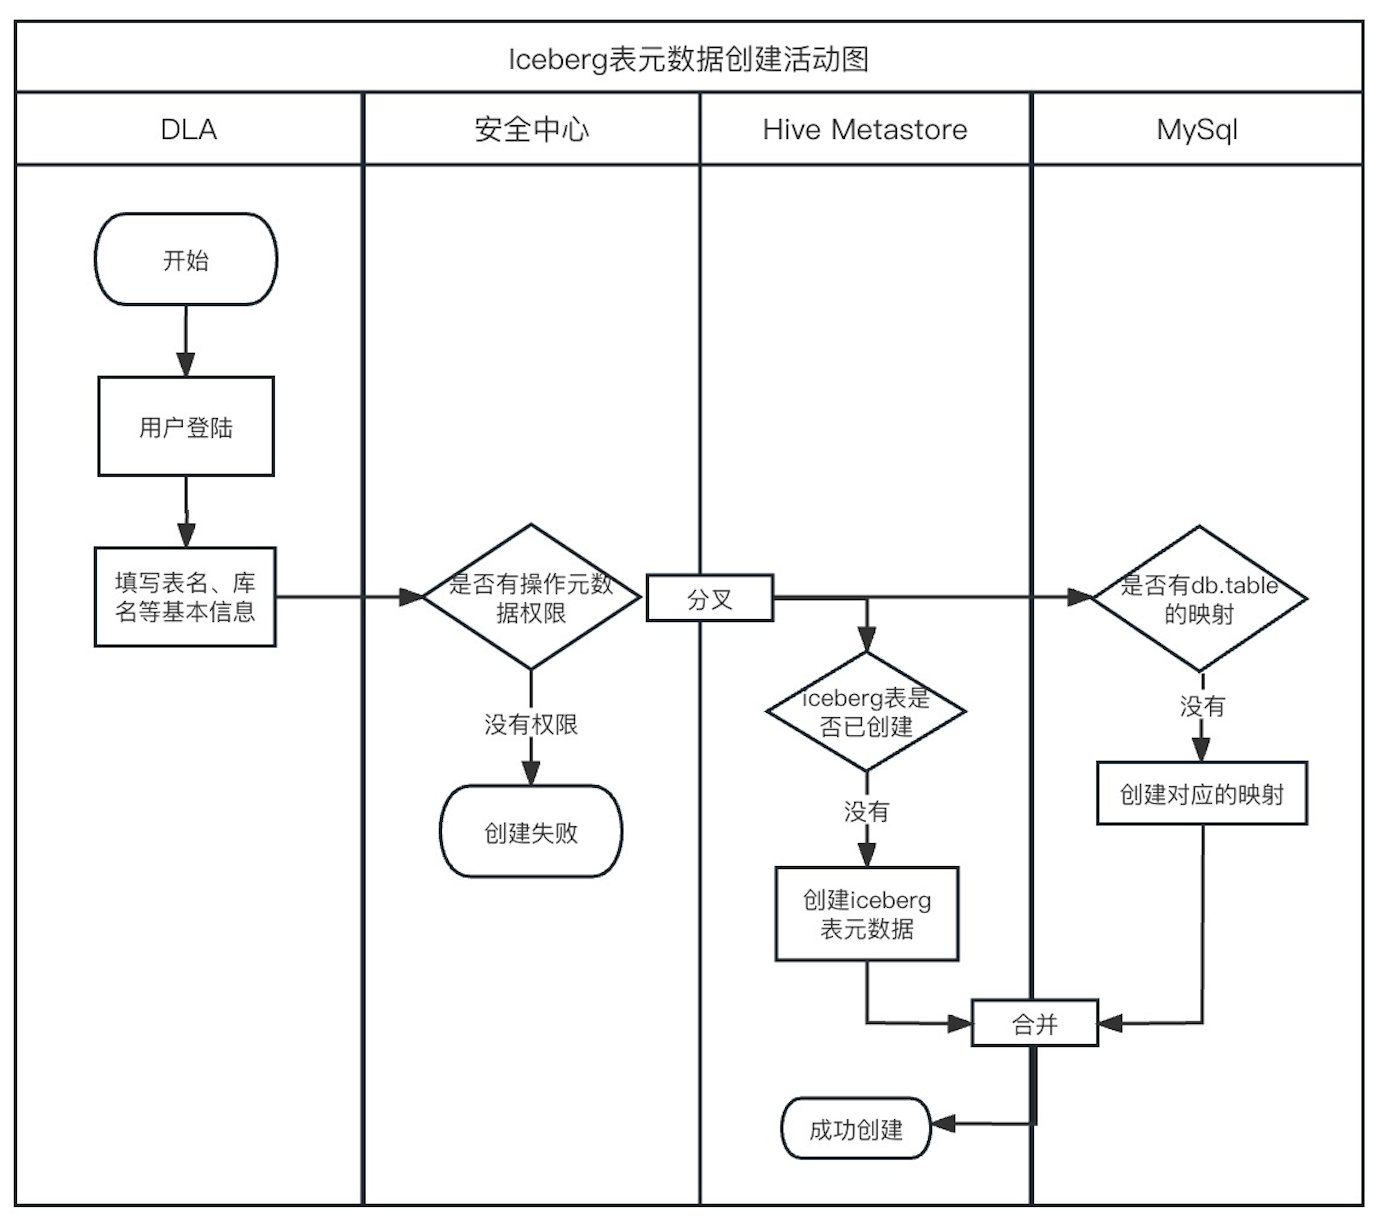
\includegraphics[width=1.0\textwidth]{表元数据创建活动图.png}
  \caption{Iceberg表元数据创建活动图}
  \label{fig:表元数据创建活动图}
\end{figure}

元数据管理系统中主要类图如图\ref{fig:MetadataControllerV2}所示:

\begin{figure}[H]
  \centering
  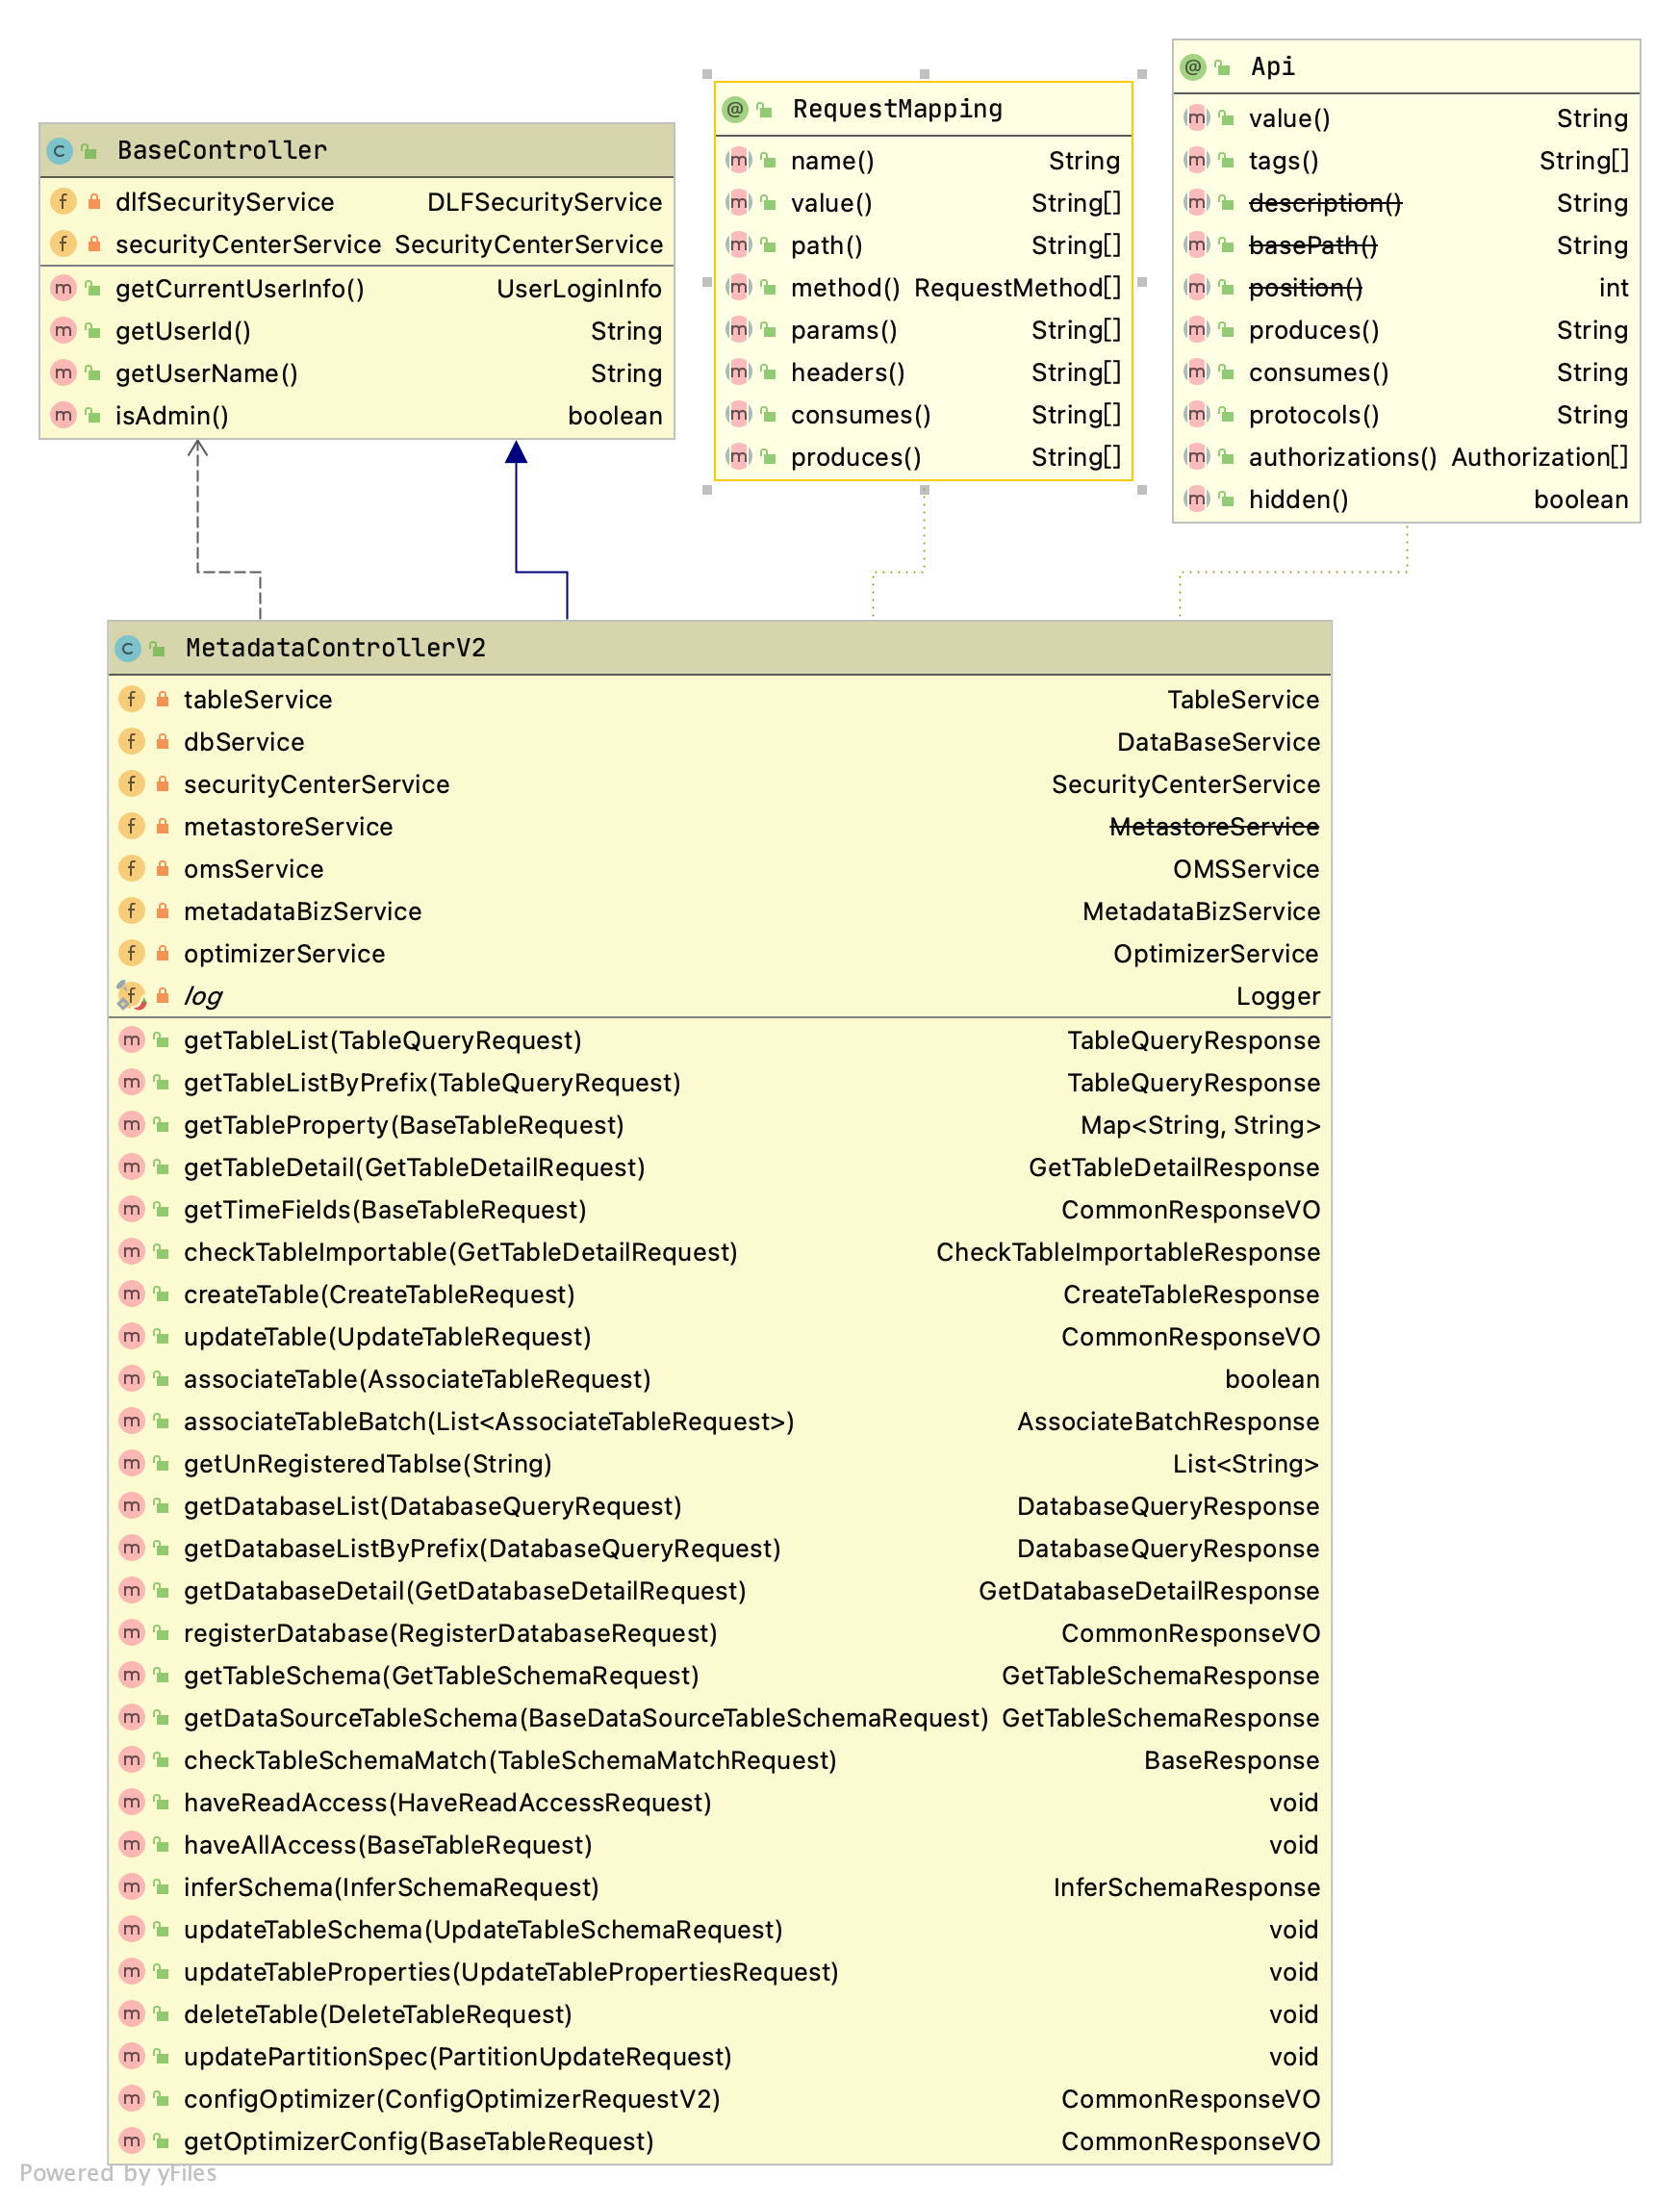
\includegraphics[width=0.95\textwidth]{MetadataControllerV2.png}
  \caption{元数据管理类图}
  \label{fig:MetadataControllerV2}
\end{figure}

MetadataControllerV2是元数据管理的核心类,是用户访问元数据管理的入口,
主要负责Iceberg表的创建、修改、查看、数据优化功能。在核心类的成员变量中,
TableService负责Iceberg表的创建、修改、查看的逻辑处理;DataBaseService
负责数据库相关操作的逻辑处理;SecurityCenterService负责安全中心认证的逻辑处理,
安全中心认证是所有操作元数据的前提,通过认证后,才能对表的结构以及数据进行查看或修改;
OMSService是元数据服务,是基于hive metastore实现的;
OptimizerService是自动优化的逻辑处理,会在后面进行详细介绍。


\section{数据入湖}

数据入湖是数据湖分析系统的核心流程功能,目的是用户通过该功能将源数据表流程化入湖
以及查看已申请入湖任务执行情况。其中入湖任务列表中具有操作任务的功能,
并且根据数据入湖方式具有不同状态展示,以供用户查看和处理。
在实时入湖场景中,DLA借助flink实现了流式增量入湖,将入湖时延降低到了分钟级(每1分钟mini-batch入湖)。

对于每一个入湖任务,都需要进行五步:
第一步是基础信息的填写,根据入湖需要选择对应的任务类型,填写必要的任务名;
第二步是填写源表的信息,其中实时入湖与关系型数据库入湖需要提前注册数据源,选择对应数据源表;
第三步是填写目标表的信息,若目标表已经创建,则会自动填充信息,若不存在,则会自动创建Iceberg表,无需提前新建表,这大大优化了入湖任务的流程;
第四步是进行映射预览,会对源表及目标表的schema进行比对,若schema不一致将无法进行下一步;
第五步是配置参数及资源。相关的活动图如图\ref{fig:任务创建活动图}所示。

\begin{figure}[H]
  \centering
  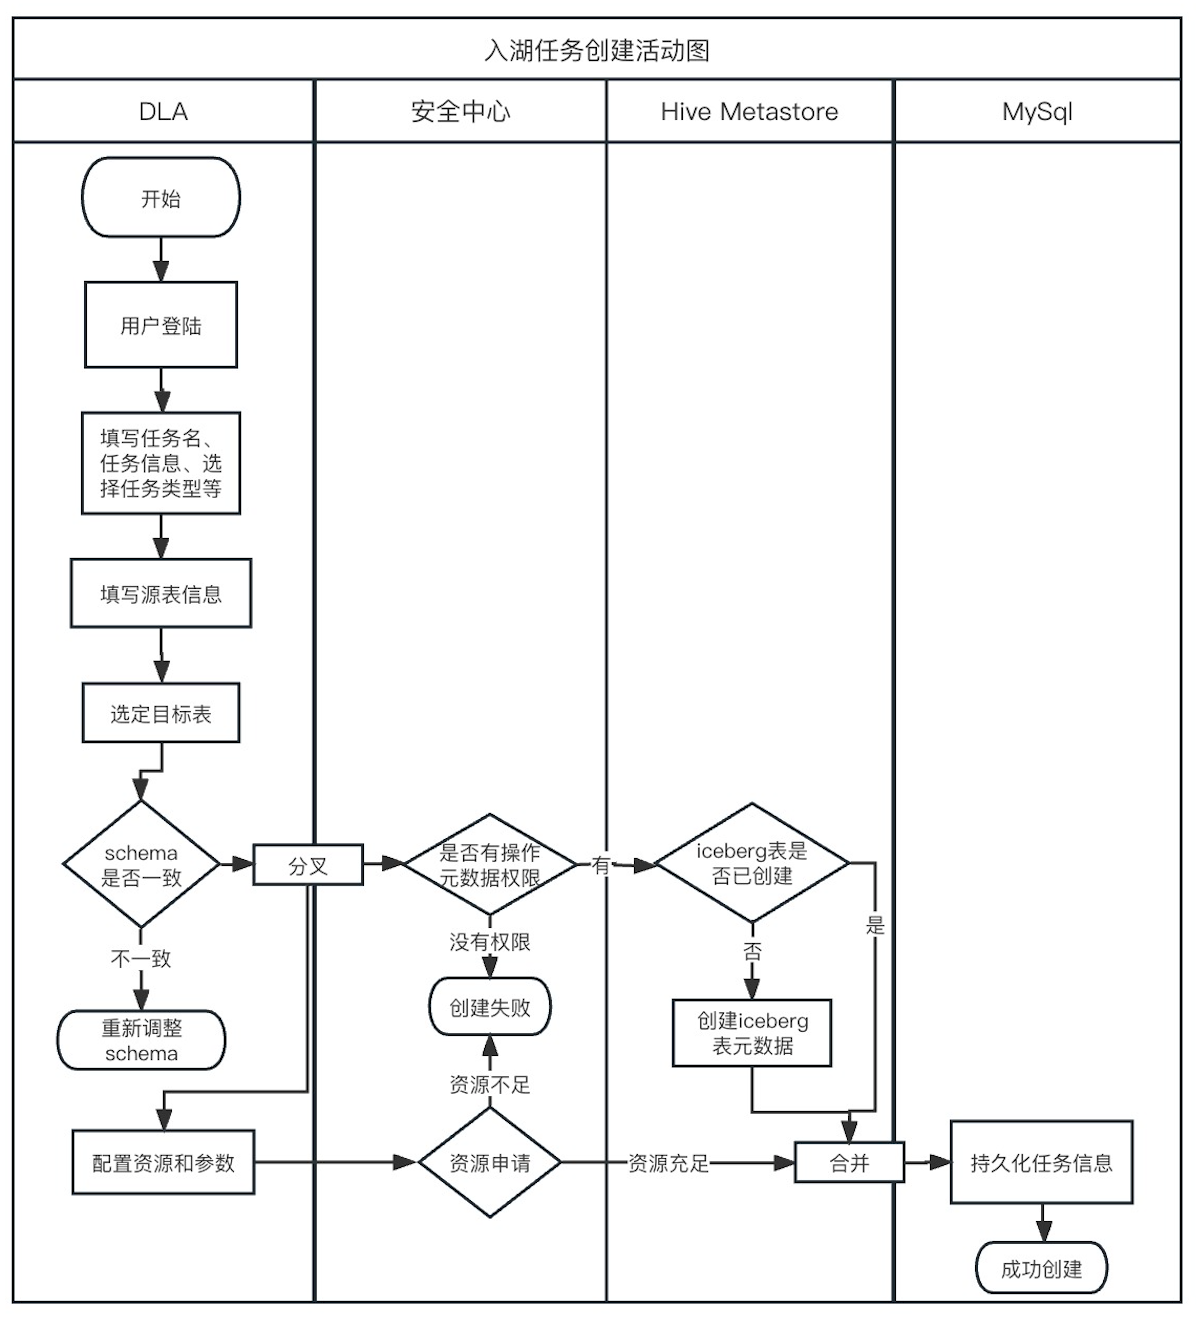
\includegraphics[width=0.87\textwidth]{任务创建活动图.png}
  \caption{入湖任务创建活动图}
  \label{fig:任务创建活动图}
\end{figure}

针对不同的任务类型,DLA分别对接了内部的不同任务平台,通过各个平台的REST API的方式实现不同任务的创建。
若为实时数据入湖任务,则会在实时流计算平台Oceanus上创建对应的实时任务来进行Iceberg表的写入,
Oceanus底层使用的引擎是flink;若为存量数据入湖或者关系
型数据入湖,则会在统一调度平台US上创建定时任务来进行Iceberg表的写入,底层使用的引擎是spark,
并且可在系统上设置时间间隔和起始时间。相关的核心类图如图\ref{fig:TaskControllerV2}所示。

\begin{figure}[H]
  \centering
  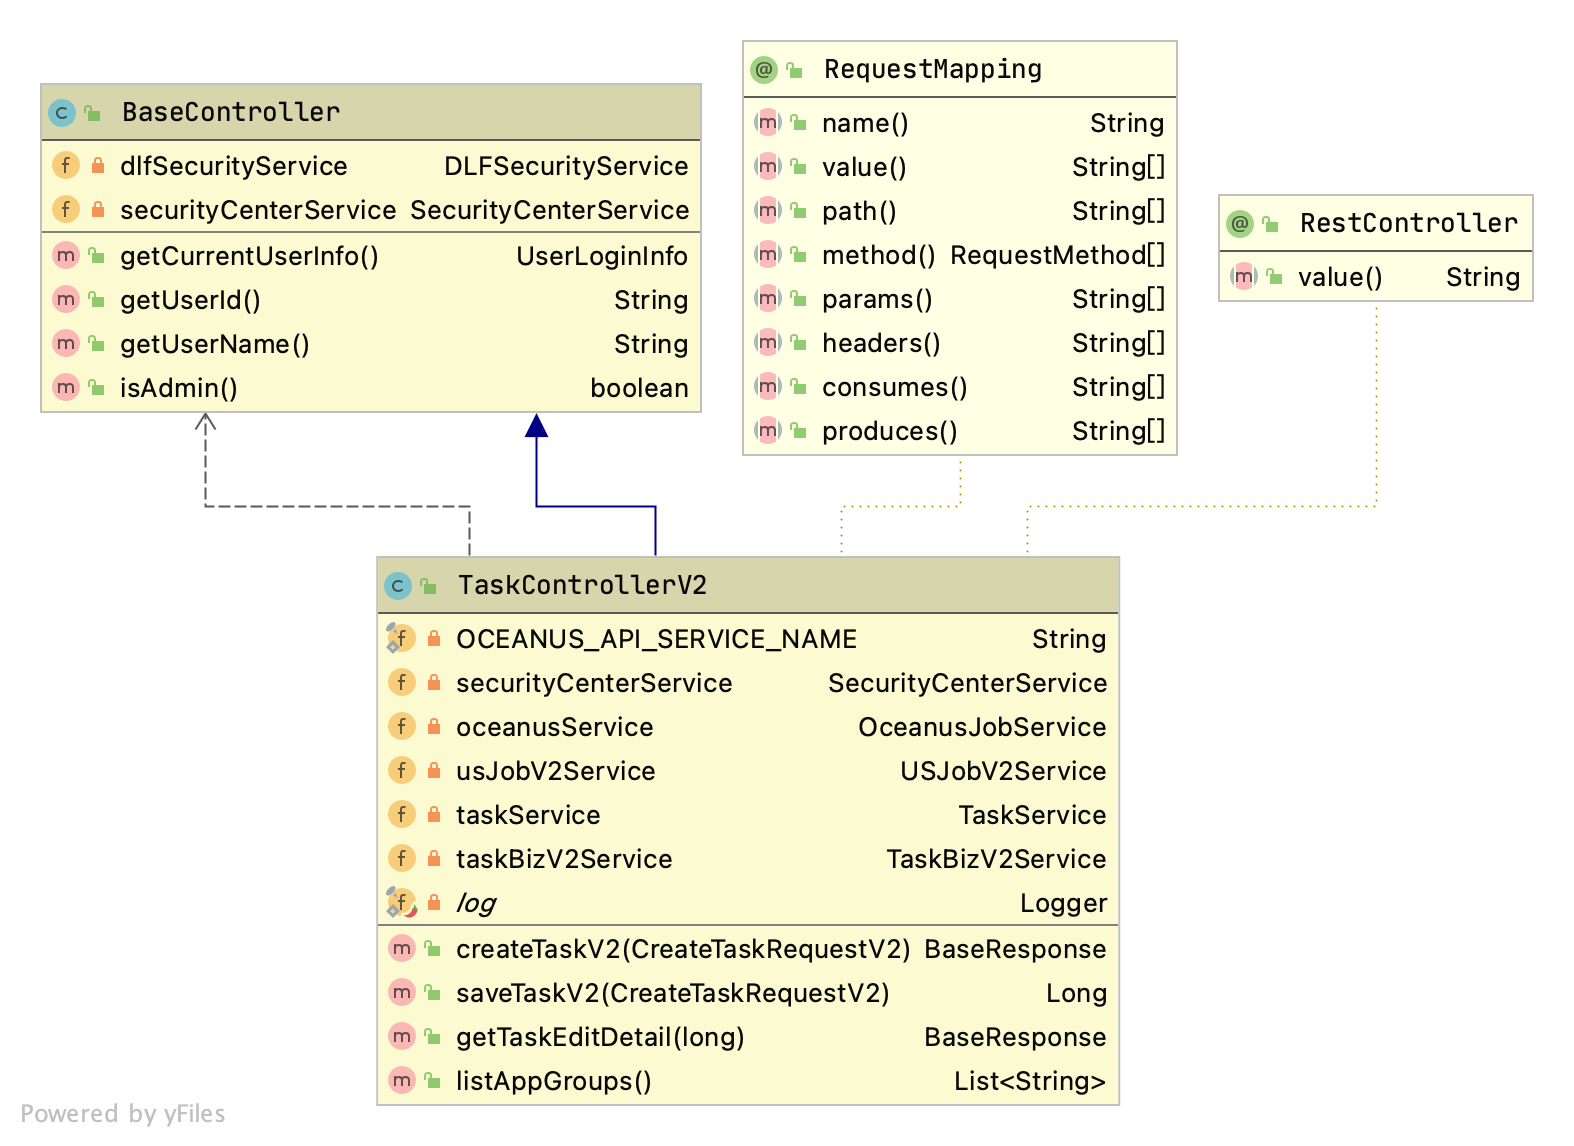
\includegraphics[width=1.0\textwidth]{TaskControllerV2.png}
  \caption{数据入湖类图}
  \label{fig:TaskControllerV2}
\end{figure}

可以看到,TaskControllerV2是数据入湖管理的核心类,是用户进行任务创建的入口,负责入湖任务的
创建、查看修改等功能,对应的逻辑处理是在TaskBizV2Service中实现的。在成员变量中,SecurityCenterService
是负责安全中心认证的;OceanusJobService是负责管理实时任务的,对接的是实时任务平台的api;
USJobV2Service是负责管理存量数据入湖任务的,对接的是统一调度平台US的api。

\section{数据探索}

数据探索是数据入湖后,用户需要进行数据查看或者数据分析时使用的工具,目前主要依赖内部的统一查询平台实现数据探索功能,
通过查询平台的SuperSQL,用户只需简单的配置参数(set supersql.execution.engine = presto / spark),
就可以轻松通过Presto或者Spark查询分析数据,其中通过presto可以进行秒级分析(查询时延平均为30s)。
SuperSQL做到计算对用户透明,
避免用户在不同系统中的切换成本和高昂的学习成本。SQL语法采用标准的SQL语法。例如图\ref{fig:presto标准sql}。
除了可以使用标准的sql进行数据探索外,统一查询平台还提供了Jupyter Notebook的方式,可以在Jupyter中使用Pyspark进行
数据的探索,该种方式与用户的交互性比较好,可以使用各种图表使数据可视化。
除了内部的统一查询平台可以进行数据探索外,数据湖分析平台还内嵌了Zeppelin来进行数据探索。

\begin{figure}[H]
  \centering
  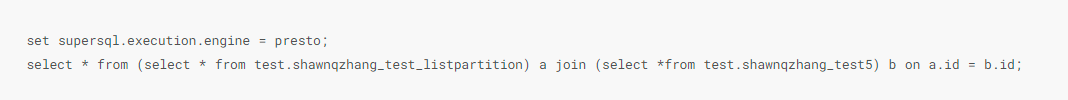
\includegraphics[width=1.0\textwidth]{presto标准sql.png}
  \caption{Presto查询sql}
  \label{fig:presto标准sql}
\end{figure}

\section{自动优化服务}

目前使用Iceberg的用户需要自己手写java代码来维护Iceberg表,
用户认为Iceberg的运维成本较高,学习成本较大,所以设计了数据自动优化服务。
数据优化服务的目的是降低用户的运维成本,使用户可以一
键启动该服务,不需要自己写java程序来优化,并会根据表的若干指标及历史执行情况
判断所需资源,并配有告警机制,及时通知专业运维处理。
当前服务包括小文件合并、历史快照清理、孤儿文件删除、数据生命周期管理等,
其中自动优化服务在小文件合并这方面做了很多的优化,会在接下来进行介绍。

在概要设计中,介绍了整个自动优化服务的总体运行流程图,根据流程图,Iceberg需要将
当前文件状态发布到外部系统,而Iceberg当前还不支持将当前文件状态发布到外部系统,
因此自动优化服务基于Iceberg的内核重新设计了不同阶段的不同事件,并针对不同的事件定义相应的指标,
通过事件汇报框架,将这些指标汇报到自动优化服务,由服务根据事件的类型来决定进行什么类型的优化和任务执行粒度。
整体事件汇报的框架如图\ref{fig:Iceberg事件汇报框架}所示,在Iceberg-core中,Iceberg Event Reporter
会将各类的Event收集并发送到一个队列中,主要收集的Event包括DDLEvent、元数据更新Event、NewSnapshotEvent等。
下游的Event处理线程会从队列中消费Event,并通过Event Listener发送给自动优化服务。在自动优化服务中,
根据不同Event所配置的规则进行相应的计算和任务调度,例如,发生了5次NewSnapshotEvent,则说明触发了
5次文件的commit操作,那么根据5次commit就执行一次小文件合并的规则,这时候就可以执行一次小文件合并,
从而提高数据查询和分析的效率。通过Iceberg Event Reporter和自动优化服务的联合使用,Iceberg可以实现
自动化的数据优化和管理,从而进一步提高Iceberg表的性能和可用性。

\begin{figure}[H]
  \centering
  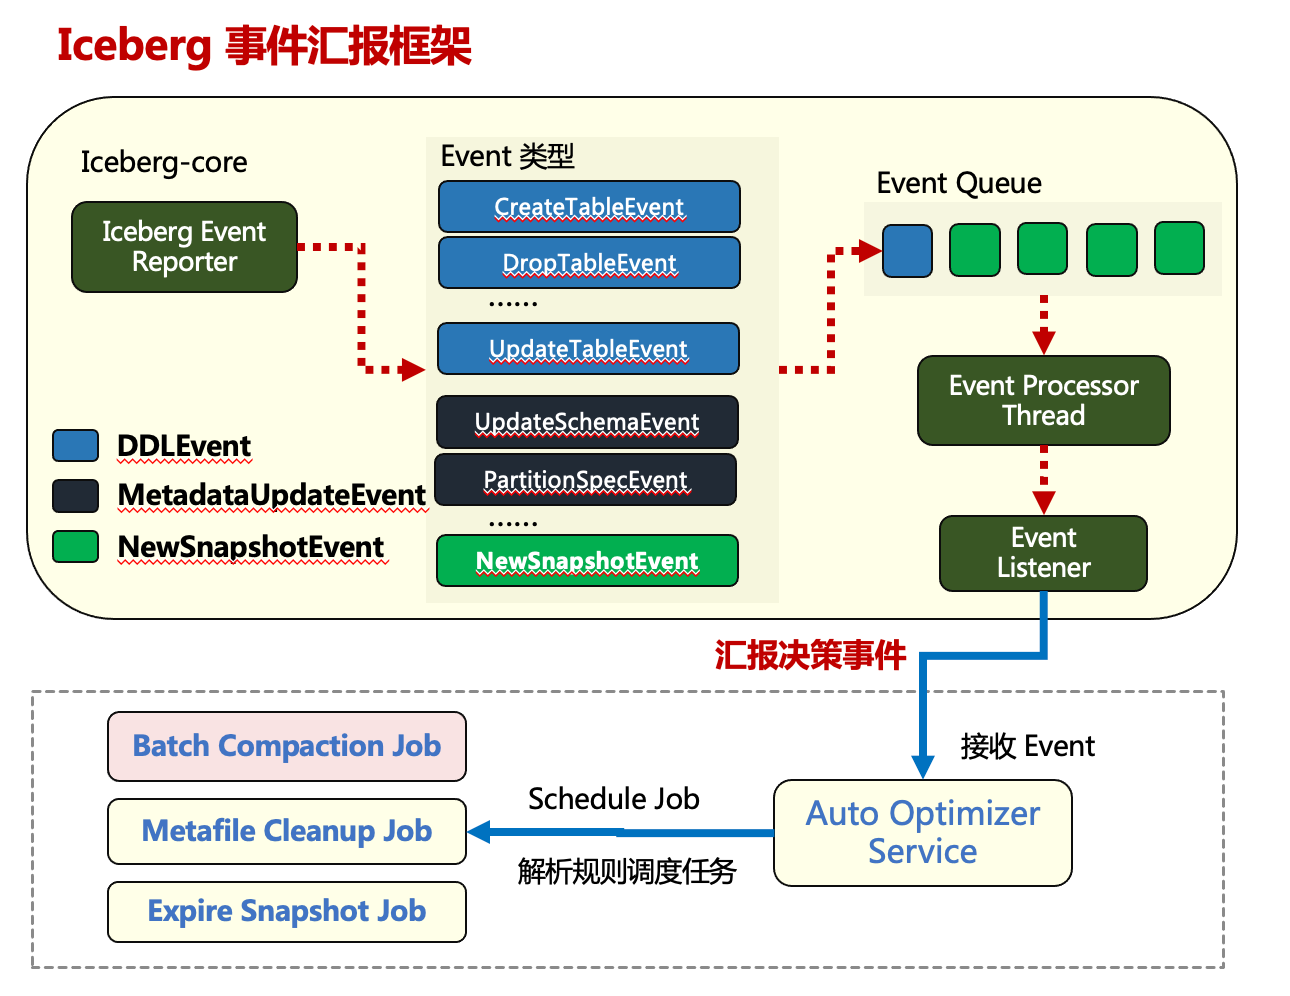
\includegraphics[width=1.0\textwidth]{Iceberg事件汇报框架.png}
  \caption{Iceberg事件汇报框架}
  \label{fig:Iceberg事件汇报框架}
\end{figure}

以NewCreateSnapshotEvent为例,如图\ref{fig:snapshot事件信息}所示,当前事件里面可以看到一个snapshot的事件信息包含新增了多少文件、
新增了多少records、新增的文件size、总的文件size等,则下游的service拿到这些event以后可以
解析开这些数据,然后配置相应的规则去触发不同的合并任务。

\begin{figure}[H]
  \centering
  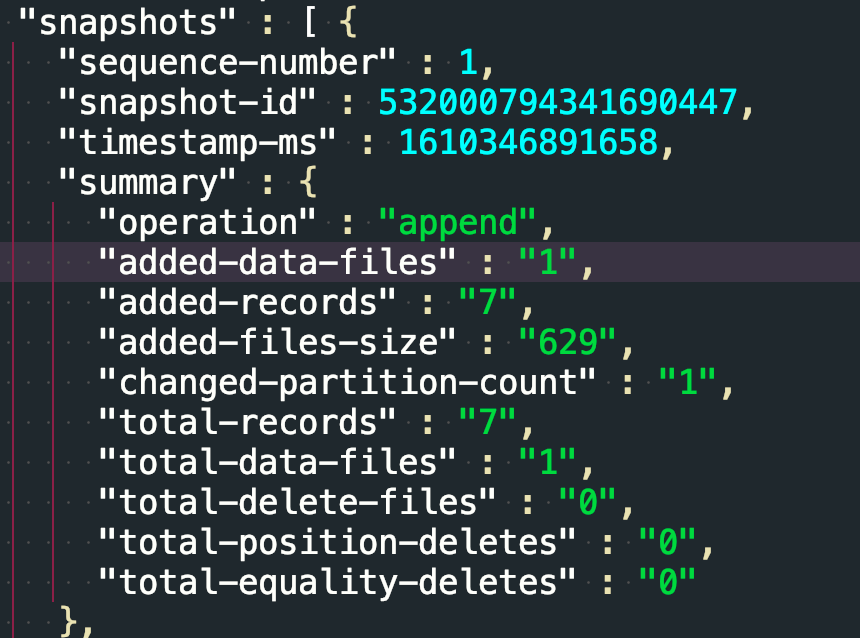
\includegraphics[width=0.67\textwidth]{snapshot事件信息.png}
  \caption{snapshot事件信息}
  \label{fig:snapshot事件信息}
\end{figure}

\subsection{合并小文件}

在概要设计中,自动优化服务决定使用均方误差(MSE)的计算方法来替代原有的小文件合并策略。这里给出详细的计算过程,
MSE通过公式\ref{eq:example1}进行计算:

\begin{equation}
  MSE=\frac {\sum_{i=1}^{N}{(Target_i - Actual_i)^2}} {N}
  \label{eq:example1}
\end{equation}

其中N代表一个分区内的文件数,Target代表合并后的目标文件大小,Actual等于min(分区内实际的文件大小, Target)。

当分区内文件状态需要更新的时候,通过公式\ref{eq:example2}和公式\ref{eq:example3}进行计算:

\begin{equation}
  SE=\sum_{i=1}^{N}{(Target_i - Actual_i)^2}
  \label{eq:example2}
\end{equation}

其中M代表分区内的新的文件数。

\begin{equation}
  MSEnew=\frac {MSEold*N+SE} {N+M}
  \label{eq:example3}
\end{equation}

阈值T的取值通过公式\ref{eq:example4}进行计算:

\begin{equation}
  T=(Target*a)^2 \qquad (0<a<1)
  \label{eq:example4}
\end{equation}

其中a需要进行配置,默认取0.75。

合并⼩⽂件主要有四个过程:

(1)根据条件(各个分区的MSE、阈值T)筛选出⽂件;

(2)根据targetSize划分task;

(3)合并⼩⽂件;

(4)返回数据到RewriteDataFilesActionResult中;

\begin{figure}[H]
  \centering
  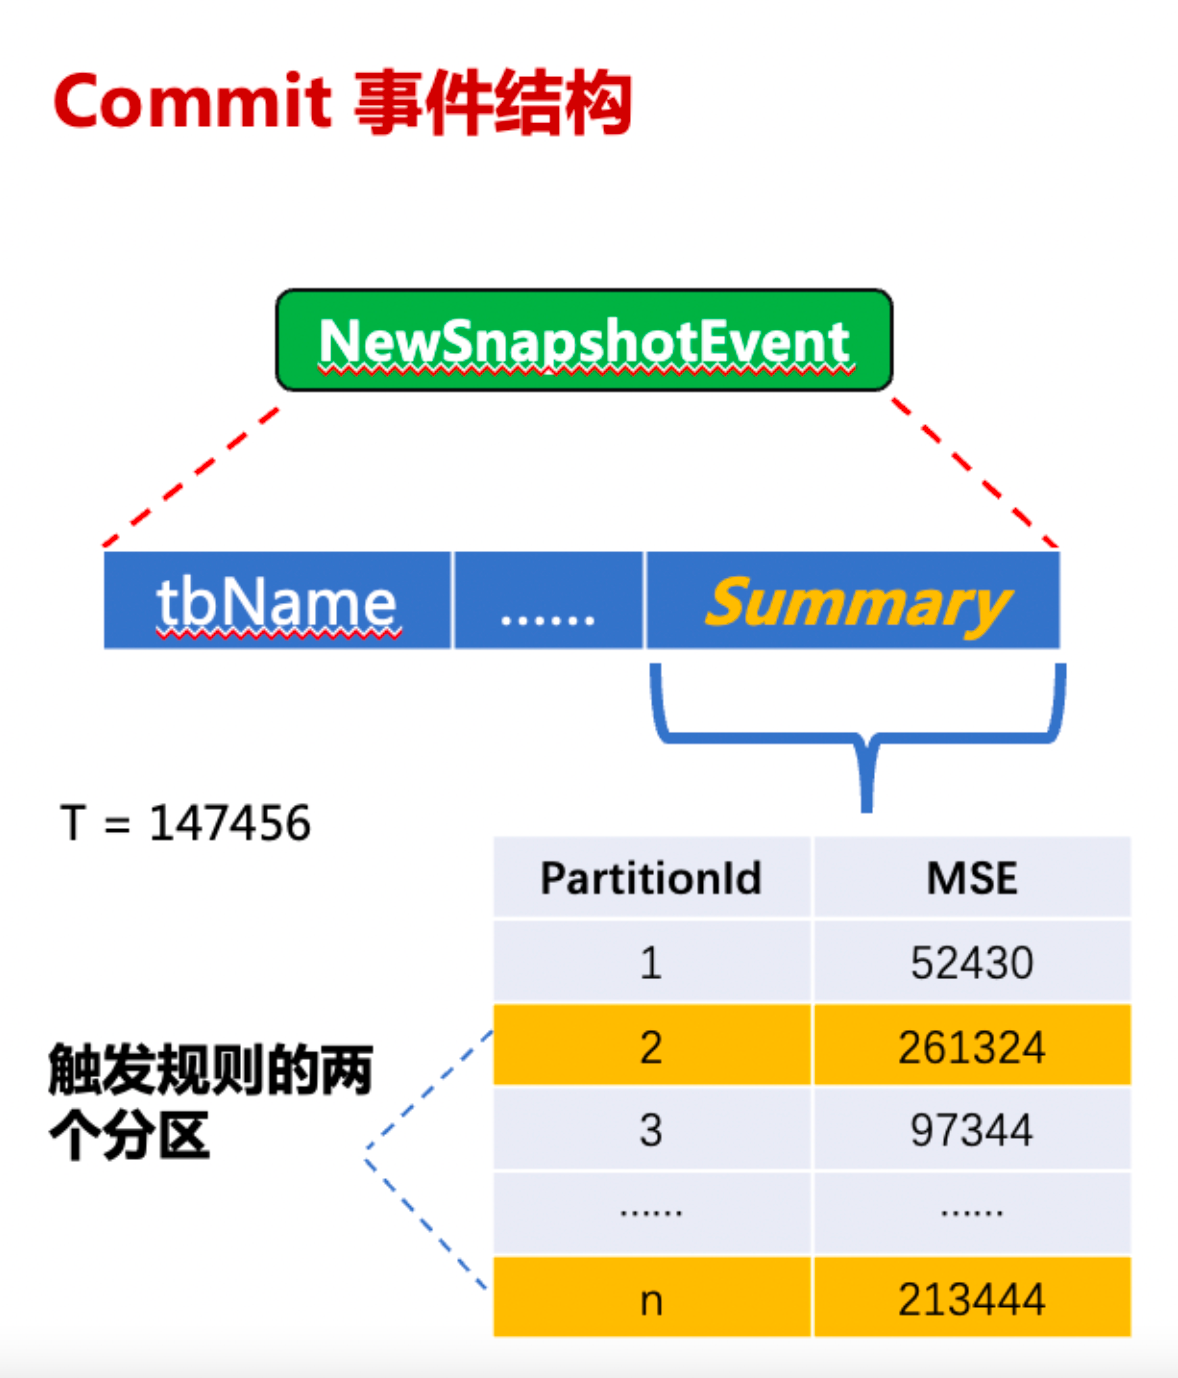
\includegraphics[width=0.4\textwidth]{Iceberg Commit事件结构.png}
  \caption{Iceberg Commit事件结构}
  \label{fig:Commit事件结构}
\end{figure}

通过公式\ref{eq:example1}~\ref{eq:example3}计算得到各个分区的MSE值之后,通过事件汇报的方式发送到文件合并服务。
后台服务在收到这些MSE值之后,
自动根据不同的表所配置的不同的值来决策是否需要对某个分区或者是某张表进行合并。 Commit事件为一次snapshot生成的事件,
通过计算每个snapshot里面的文件状态并通过summary的方式记录,通过事件发送到后端服务。这样,服务可以清楚地了解当前
每一张表的snapshot中的文件状态,以此作为是否触发合并的判断依据。Iceberg Commit事件结构如图\ref{fig:Commit事件结构}所示,可以看到
Summary中记录了每个分区的MSE值。与阈值T进行比较后,发现分区2和分区n的MSE大于T,因此触发了合并任务。通过
这种方式,Iceberg可以自动地进行文件合并,从而优化数据查询和分析的性能和效率。

\begin{figure}[H]
  \centering
  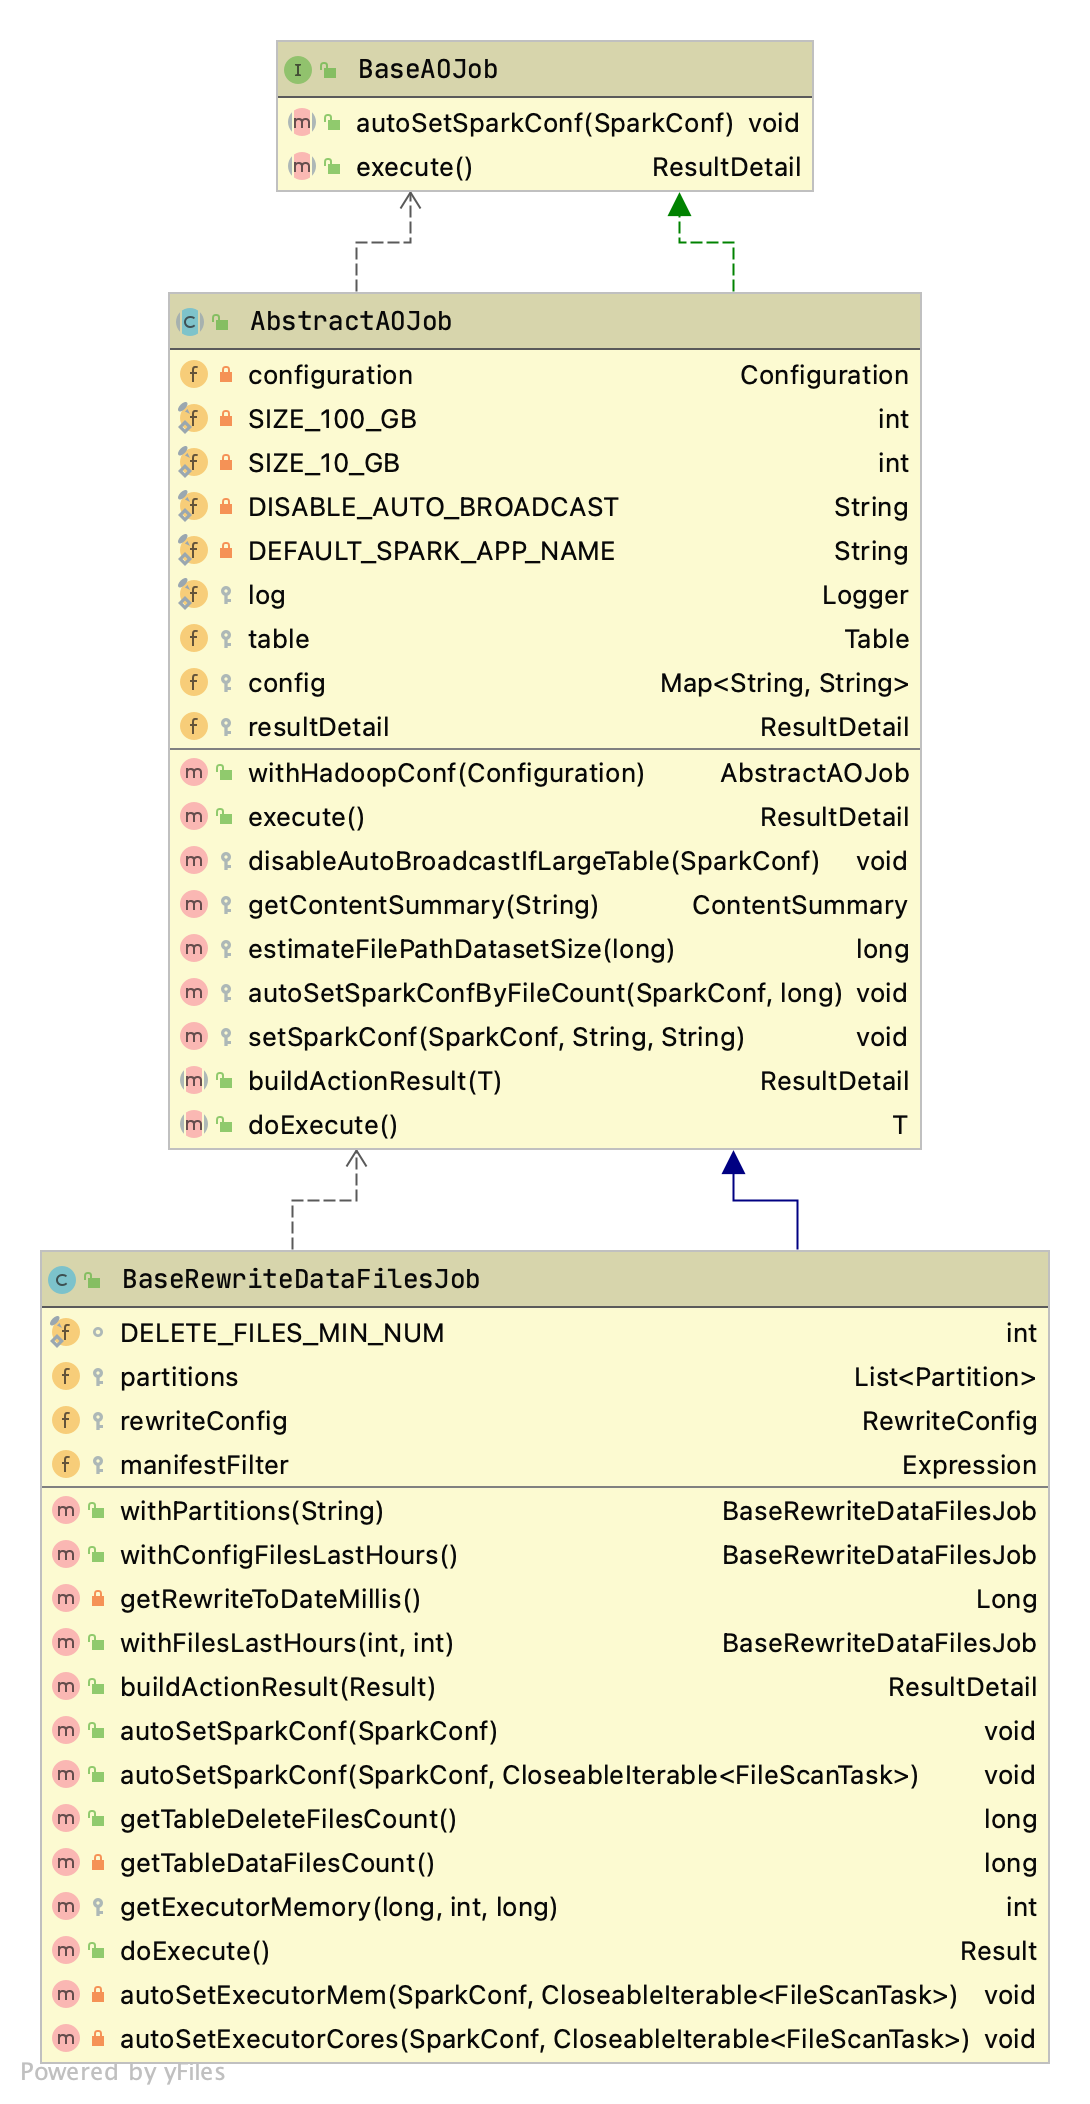
\includegraphics[width=0.8\textwidth]{BaseRewriteDataFilesJob.png}
  \caption{小文件合并相关类图}
  \label{fig:BaseRewriteDataFilesJob}
\end{figure}

小文件合并相关的类图如图\ref{fig:BaseRewriteDataFilesJob}所示。MSE是针对每个分区进行计算的,所有会有一个存放partition的list;
RewriteConfig是用于配置参数修改的,比如目标文件的大小、计算阈值T的比例系数等;
buildActionResult会将表名、size大小、删除的文件、增加的文件封装起来交给下游的指标系统;
doExecute会调用Iceberg那边提供的重写文件接口进行实际的文件合并操作。

经过这样的优化后。如图\ref{fig:不同时刻作业合并小文件数},和之前的定时调度进行合并小文件相比,可以看到基于MSE的小文件合并在文件数量上得到了很好的平衡。
如图\ref{fig:随着时间的执行小文件个数的变化}所示,合并优化的文件状态均在一个均衡的水平,
小文件的增长得到了有效的控制,在3841号快照之前,小文件数量一直上升,这是因为离线合并任务检查MSE的时间粒度为5分钟,
在这之后时间粒度改为1分钟,又在快照8065之后改为30秒,这是因为在之前的合并任务检查MSE时,发现MSE远大于设定的阈值,
于是降低MSE检查的时间粒度,以便更早地发现MSE值已达到阈值,从而触发合并任务。

\begin{figure}[H]
  \centering
  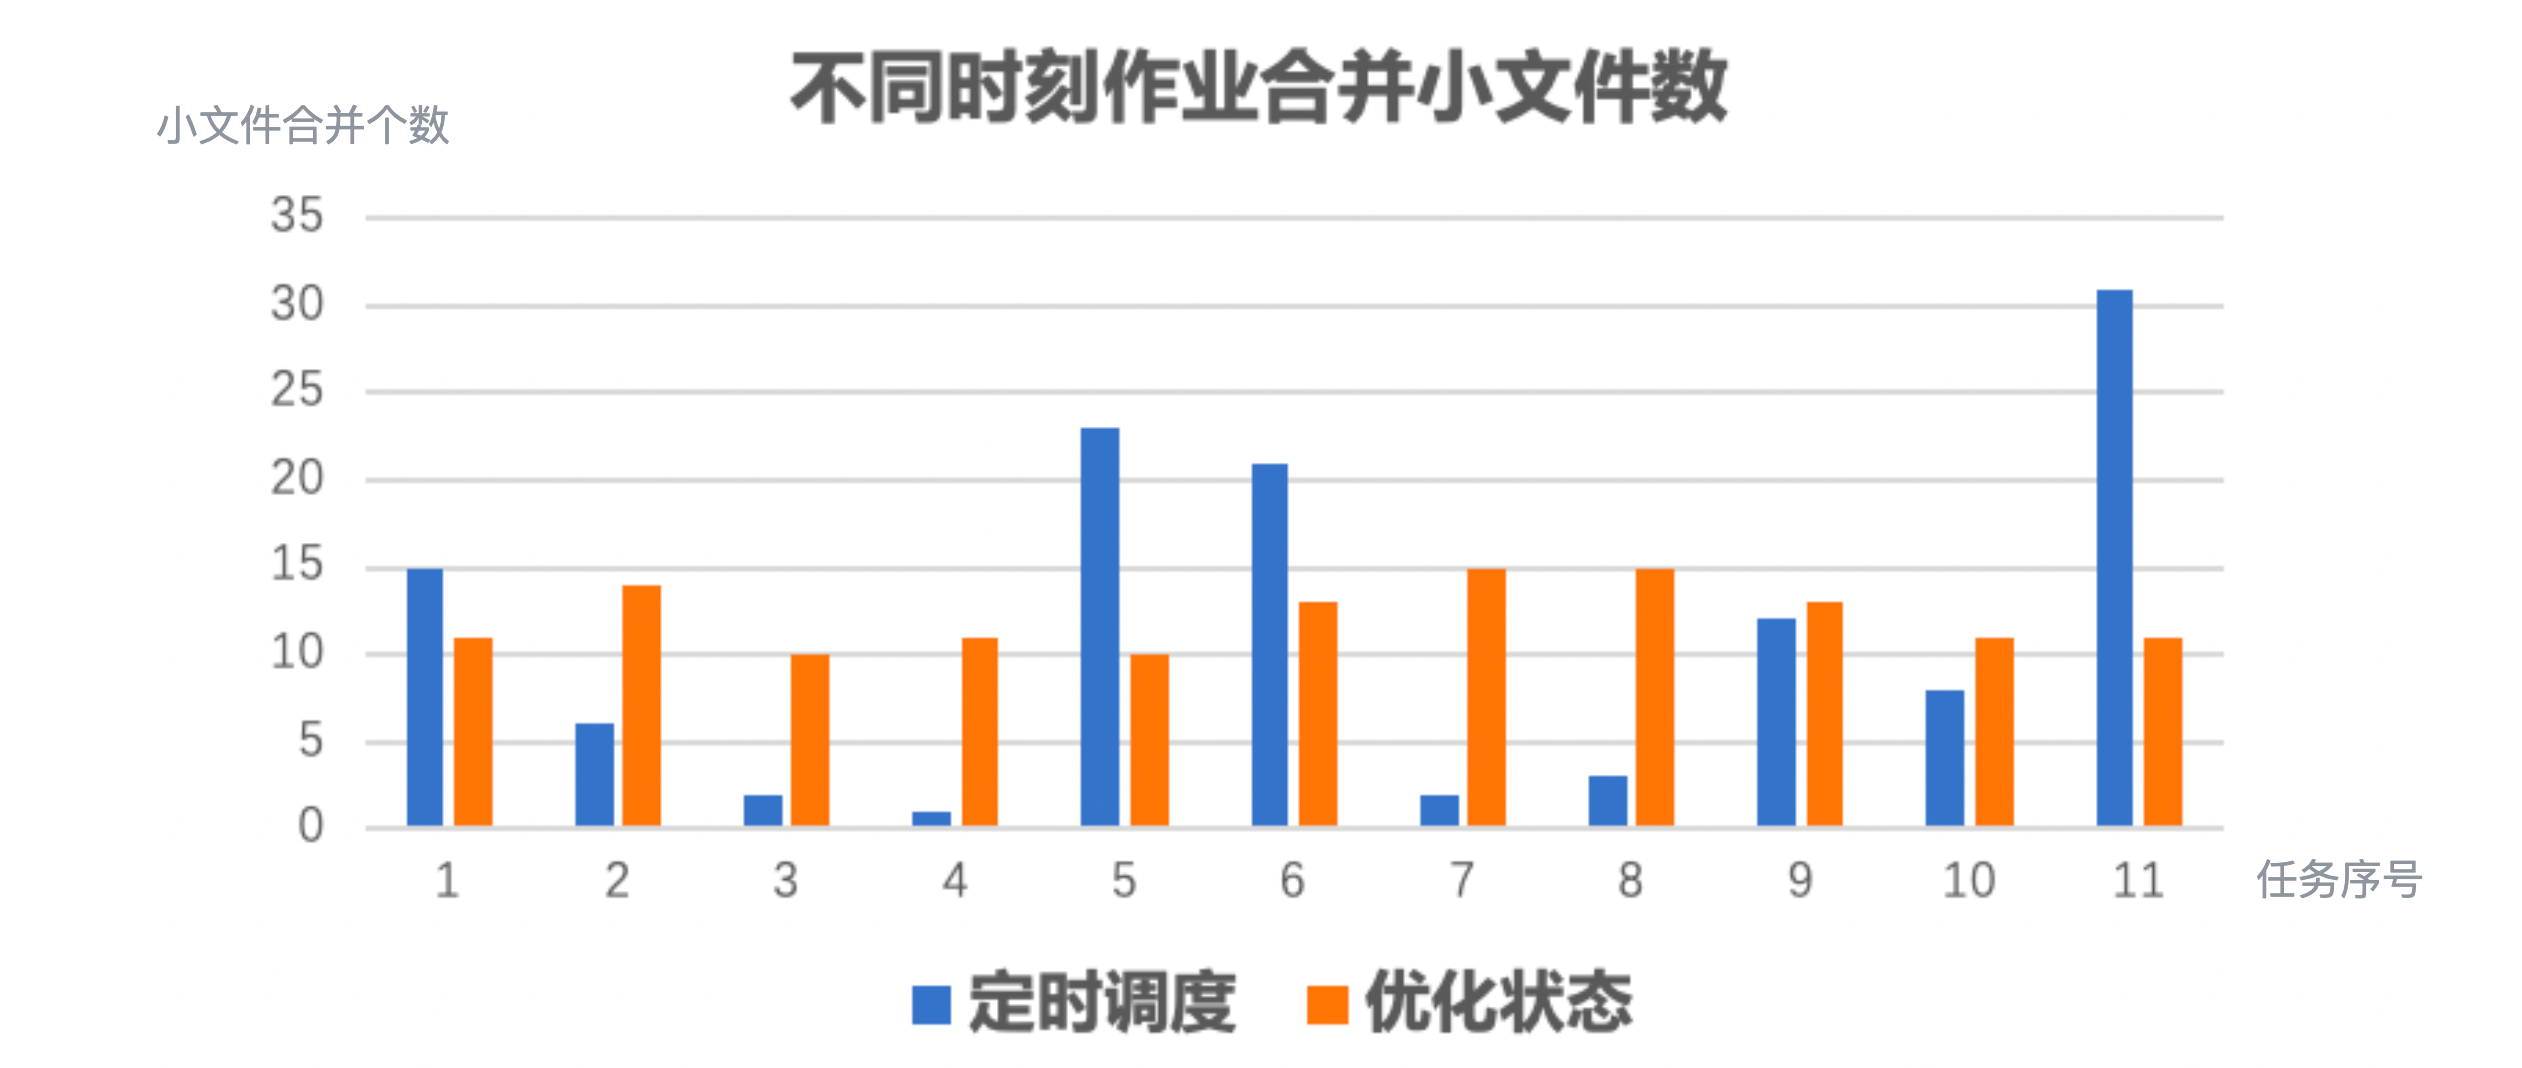
\includegraphics[width=1.0\textwidth]{不同时刻作业合并小文件数.png}
  \caption{不同时刻作业合并小文件数}
  \label{fig:不同时刻作业合并小文件数}
\end{figure}

\begin{figure}[H]
  \centering
  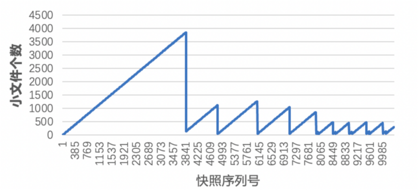
\includegraphics[width=1.0\textwidth]{随着时间的执行小文件个数的变化.png}
  \caption{随着时间的执行小文件个数的变化}
  \label{fig:随着时间的执行小文件个数的变化}
\end{figure}

\subsection{历史快照清理}

对于历史快照清理,自动优化服务设置了两个参数来控制快照删除,分别是dla.optimizer.expire.snapshot.seconds
和dla.optimizer.expire.snapshot.num,表示快照失效时间和快照保留数量,达到任何一个条件都将进行快照的清除。
被删除的snapshot将不能进⾏time travel(时间旅⾏),
当将元数据中的cleanExpiredFiles设置为true,物理⽂件也将被删除;
ExpireSnapshot删除过期快照步骤有两步:

(1)调⽤RemoveSnapshots的commit删除快照,当cleanExpiredFiles设置为true时删除对应的物理⽂件;

(2)将数据写⼊到result中。

历史快照清理的相关类图如图\ref{fig:ExpireSnapshotsJob}所示。
buildActionResult会将表名、删除的dataFiles、删除的manifestFiles、删除的manifestLists封装起来交给下游的指标系统;
doExecute会调用Iceberg那边提供的文件清除接口进行实际的文件删除操作。

\begin{figure}[H]
  \centering
  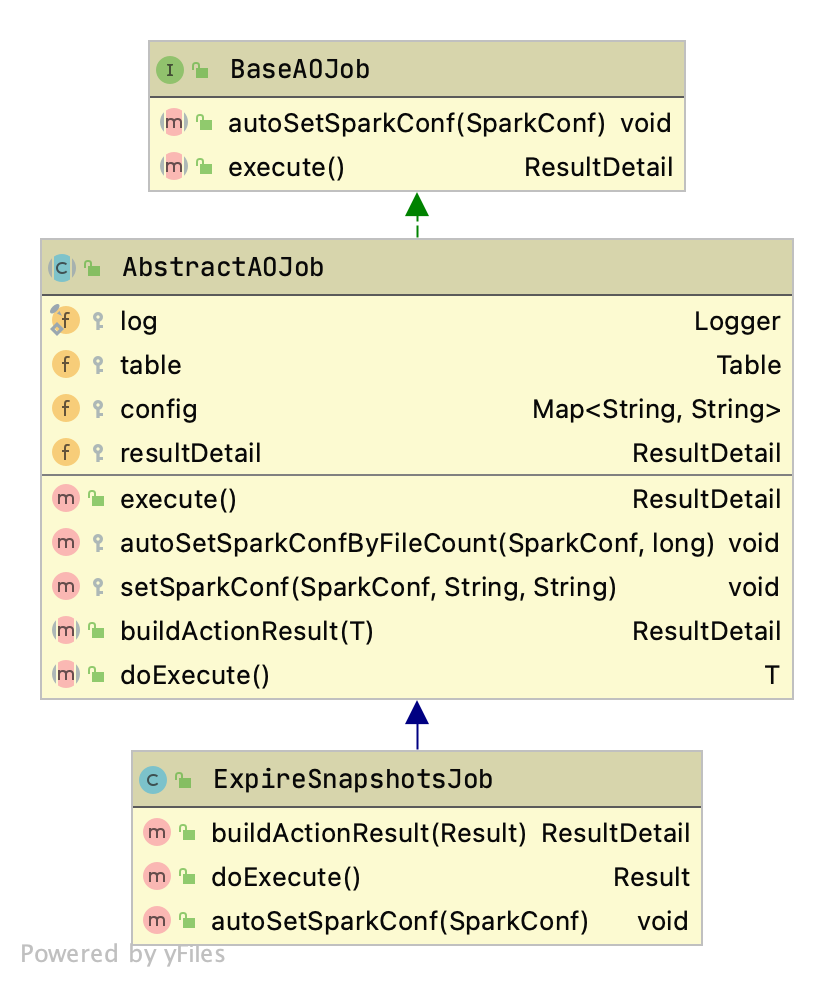
\includegraphics[width=0.82\textwidth]{ExpireSnapshotsJob.png}
  \caption{历史快照清理相关类图}
  \label{fig:ExpireSnapshotsJob}
\end{figure}

\subsection{孤儿文件删除}

清理孤⼉⽂件过程分为三步:

(1)筛选出合规的数据⽂件(数据及元数据)validFileDF,通过⽂件fs client(hdfs/cos)
筛出过期的⾮隐藏⽂件(以下划线和点开头的⽂件)actualFileDF;

(2)将actualFileDF与validFileDF和他们相交的公共部分joinCond做left anti join,最终的⽂件即orphanFiles,并将此⽂件序列删除;

(3)将删除结果写⼊到DeleteOrphanFiles.Result中。

孤儿文件删除的相关类图如图\ref{fig:孤儿文件删除相关类图}所示。
buildActionResult会将删除的文件封装起来交给下游的指标系统;
doExecute会调用Iceberg那边提供的删除孤儿文件接口进行实际的文件删除操作。

\begin{figure}[H]
  \centering
  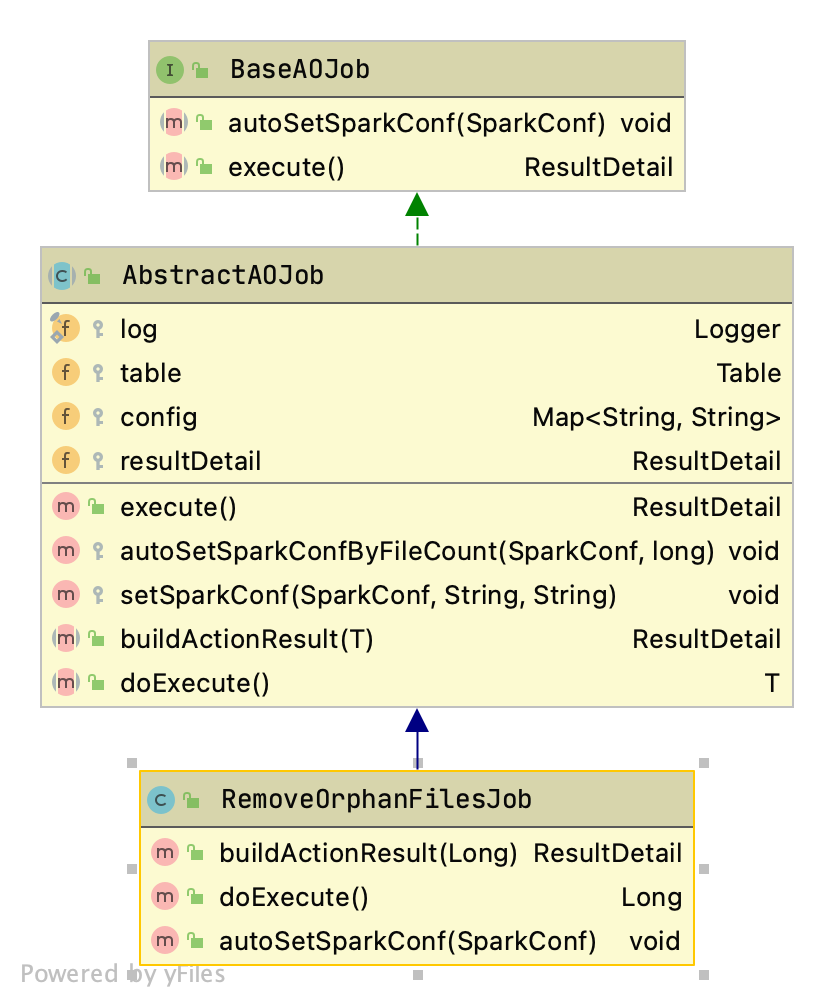
\includegraphics[width=0.75\textwidth]{RemoveOrphanFilesJob.png}
  \caption{孤儿文件删除相关类图}
  \label{fig:孤儿文件删除相关类图}
\end{figure}

\subsection{数据生命周期管理}

对于生命周期管理,需要用户设置时间字段timeField和过期时间expireTime,这就要求table schema
中有时间相关的字段,然后在实际运行时会根据每条数据的timeField的值和设置的expireTime进行比较,然后决定是否进行数据的删除。
生命周期管理的过程分为四步:

(1)扫描获取所有的dataFile;

(2)读取upperBounds中对应字段的值(dataFile中记录字段最大值);

(3)计算过期时间最大值:ExpiredTime = dataStartTime - (durationInDays * millisecondInDays),
如果ExpiredTime > upperBounds(field.fieldId()),大于则将此dataFile添加到deleteFile文件序列中;

(4)将deleteFile文件commit。

\begin{figure}[H]
  \centering
  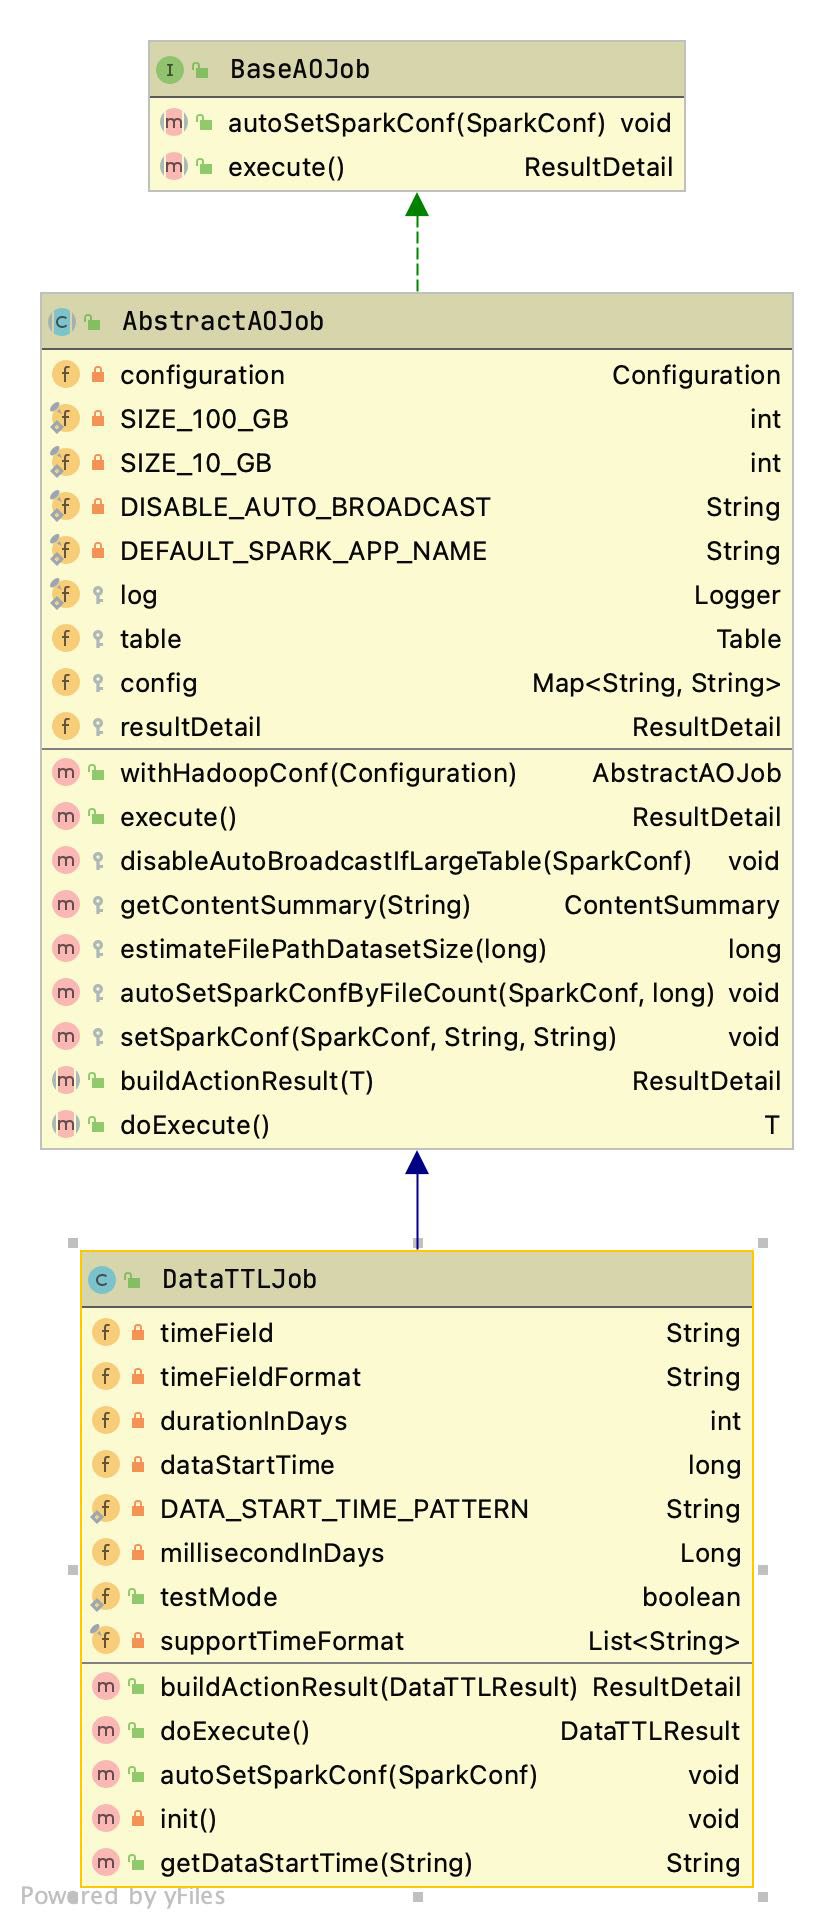
\includegraphics[width=0.7\textwidth]{dataTTLJob.png}
  \caption{生命周期管理相关类图}
  \label{fig:dataTTLJob}
\end{figure}

孤儿文件删除的相关类图如图\ref{fig:dataTTLJob}所示。timeField是所选的时间字段,timeFieldFormat是时间的格式;
durationInDays是数据持续的时间,需要用户设置,用来和dataStartTime计算得到ExpiredTime;
getDataStartTime是获取dataStartTime的,是任务启动时的时间;
buildActionResult会将删除的数据条数和失效时间封装起来交给下游的指标系统;
doExecute会根据上面的过程进行实际的数据删除操作。

\section{本章小结}

本章主要介绍了系统的详细设计,利用类图和活动图,对数据源管理、元数据管理、数据入湖、数据探索、自动优化服务
实现过程中的重难点进行了详细的阐述。
